\documentclass[11pt,a4paper]{article}
\usepackage[utf8]{inputenc}
\usepackage[T1]{fontenc}
\usepackage[margin=1in]{geometry}
\usepackage{amsmath}
\usepackage{amssymb}
\usepackage{graphicx}
\usepackage{hyperref}
\usepackage{listings}
\usepackage{xcolor}
\usepackage{tikz}
\usepackage{pgfplots}
\usepackage{pgfplotstable}
\usepackage{booktabs}
\usepackage{array}
\usepackage{tabularx}
\usepackage{multirow}
\usepackage{fancyhdr}
\usepackage{mdframed}
\usepackage{tcolorbox}
\usepackage{float}

\pgfplotsset{compat=1.18}
\usetikzlibrary{shapes,arrows,arrows.meta,positioning,calc,decorations.pathreplacing,
                decorations.markings,patterns,fit,backgrounds,shadows}

% ─── Colours ─────────────────────────────────────────────────────────────────
\definecolor{qugblue}{RGB}{30,100,200}
\definecolor{qugred}{RGB}{200,50,50}
\definecolor{quggreen}{RGB}{50,160,80}
\definecolor{qugorange}{RGB}{220,120,20}
\definecolor{qugpurple}{RGB}{120,50,180}
\definecolor{qugdark}{RGB}{20,30,50}
\definecolor{lightgray}{RGB}{245,245,250}
\definecolor{warnyellow}{RGB}{255,200,50}
\definecolor{codeblue}{RGB}{40,80,160}

% ─── Code listings ───────────────────────────────────────────────────────────
\lstdefinelanguage{Rust}{
  keywords={fn,let,mut,if,else,match,return,Ok,Err,Some,None,true,false,
             async,await,pub,use,mod,struct,impl,enum,trait,for,while,loop,
             in,break,continue,move,ref,as,where,type,const,static,unsafe,
             self,Self,super,crate,extern,dyn,box},
  sensitive=true,
  morecomment=[l]{//},
  morecomment=[s]{/*}{*/},
  morestring=[b]",
}

\lstset{
  basicstyle=\ttfamily\footnotesize,
  breaklines=true,
  frame=single,
  rulecolor=\color{qugblue!40},
  backgroundcolor=\color{lightgray},
  keywordstyle=\color{codeblue}\bfseries,
  commentstyle=\color{gray}\itshape,
  stringstyle=\color{qugred},
  numbers=left,
  numberstyle=\tiny\color{gray},
  numbersep=5pt,
  language=Rust,
  literate={->}{{\texttt{->}}}2 {=>}{{\texttt{=>}}}2,
  extendedchars=true,
  inputencoding=utf8
}

% ─── Headers ─────────────────────────────────────────────────────────────────
\pagestyle{fancy}
\fancyhf{}
\fancyhead[L]{\small\textcolor{qugblue}{\textbf{Q-NarwhalKnight}}}
\fancyhead[R]{\small\textcolor{gray}{Balance Incident Report — April 29, 2026}}
\fancyfoot[C]{\small\thepage}

% ─── Notice box ──────────────────────────────────────────────────────────────
\tcbuselibrary{breakable,skins}
\newtcolorbox{noticebox}[1][]{
  enhanced, breakable,
  colback=qugred!5, colframe=qugred!60,
  fonttitle=\bfseries, title={#1},
  arc=4pt, boxrule=1pt
}
\newtcolorbox{infobox}[1][]{
  enhanced, breakable,
  colback=qugblue!5, colframe=qugblue!60,
  fonttitle=\bfseries, title={#1},
  arc=4pt, boxrule=1pt
}
\newtcolorbox{fixbox}[1][]{
  enhanced, breakable,
  colback=quggreen!5, colframe=quggreen!60,
  fonttitle=\bfseries, title={#1},
  arc=4pt, boxrule=1pt
}

% ─── Document ─────────────────────────────────────────────────────────────────
\title{%
  \vspace{-1em}%
  {\Large\textbf{Q-NarwhalKnight: Balance Incident Report}}\\[0.4em]
  {\large Post-Mortem — April 29, 2026}\\[0.6em]
  {\normalsize QUGUSD$\to$QUG Swap Revert \& Post-Checkpoint Balance Wipe}\\[0.3em]
  {\small\textcolor{gray}{Version 10.5.2 Incident Analysis \& Resolution}}
}
\author{Q-NarwhalKnight Development Team}
\date{April 29, 2026}

\begin{document}

\maketitle
\thispagestyle{fancy}

% ─── ABSTRACT ────────────────────────────────────────────────────────────────
\begin{abstract}
\noindent
On April 29, 2026, two related bugs were discovered and resolved in the
Q-NarwhalKnight network. The first caused QUGUSD$\to$QUG native swaps to silently
revert the user's QUG balance 2--3 minutes after execution, making swaps appear
to fail. The second, revealed when fixing the first, caused native QUG balances
accumulated via those swaps to disappear after a node restart.
We document both bugs with full root-cause traces, the fixes shipped in
\textbf{v10.5.1} and \textbf{v10.5.2}, a correctness analysis, and the remaining
architectural gaps. This document is published transparently because users could
observe their balances change on-screen and deserve a complete explanation.
\end{abstract}

\tableofcontents
\newpage

% ═════════════════════════════════════════════════════════════════════════════
\section{Executive Summary}
% ═════════════════════════════════════════════════════════════════════════════

\begin{noticebox}[What Users Observed]
\begin{enumerate}
  \item After swapping QUGUSD $\to$ native QUG, the wallet UI showed the correct
        new balance immediately — then silently reverted to the old value within
        approximately 2--3 minutes.
  \item After a network node restart on April 29, several users who had
        successfully accumulated QUG via swaps found their balances lower than
        expected. In the most visible case, a user who had 735 QUG before the
        restart saw their balance drop to 648 QUG — a loss of 87 QUG.
\end{enumerate}
Both behaviours stemmed from the same underlying root cause: the swap handler
wrote QUG credits to an in-memory cache but failed to persist them to the
correct durable storage location.
\end{noticebox}

\medskip

\begin{fixbox}[Resolution]
\textbf{v10.5.1} (same day) fixed the swap revert bug by writing the QUG credit
directly to the authoritative RocksDB column family (\texttt{CF\_MANIFEST}) in
the HTTP handler.  \textbf{v10.5.2} fixed the restart credit-loss bug by (a)
resetting the DEX idempotency counter on checkpoint restore and (b) removing an
incorrect write that caused the startup adjustment routine to compute a zero
delta.  A third change adds an \emph{authoritative-node guard} that prevents
any future checkpoint from wiping an already-populated genesis node.
\end{fixbox}

% ═════════════════════════════════════════════════════════════════════════════
\section{Storage Architecture Overview}
% ═════════════════════════════════════════════════════════════════════════════

The node stores wallet balances across two independent RocksDB column families
and an in-memory map.  Understanding this structure is essential to following
the bug trace.

\begin{figure}[H]
\centering
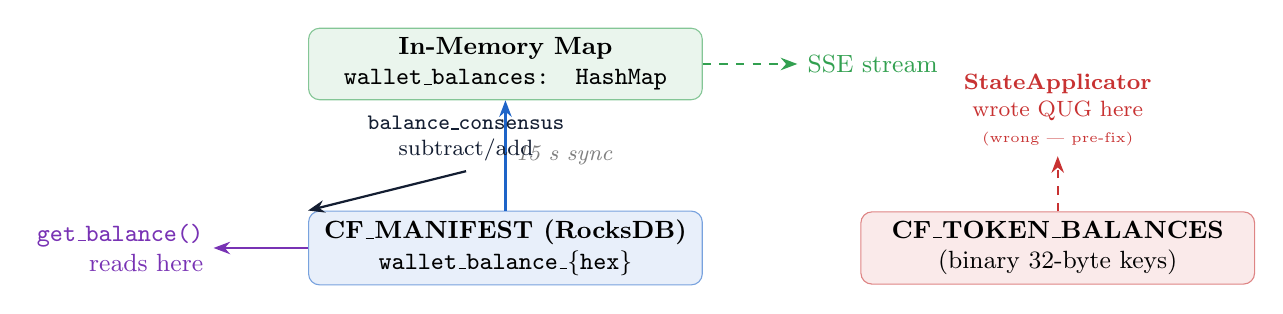
\begin{tikzpicture}[
  node distance=0.8cm and 1.6cm,
  box/.style={rectangle, rounded corners=4pt, draw, minimum width=3.6cm,
              minimum height=0.9cm, font=\small, align=center},
  dbbox/.style={box, fill=qugblue!10, draw=qugblue!60},
  membox/.style={box, fill=quggreen!10, draw=quggreen!60},
  badbox/.style={box, fill=qugred!10, draw=qugred!60},
  arrow/.style={-{Stealth[length=6pt]}, thick},
  label/.style={font=\footnotesize\itshape, text=gray}
]

% In-memory
\node[membox, minimum width=5cm] (inmem) {\textbf{In-Memory Map}\\
  \texttt{wallet\_balances: HashMap}};

% CF_MANIFEST
\node[dbbox, minimum width=5cm, below=1.4cm of inmem] (cfm) {%
  \textbf{CF\_MANIFEST (RocksDB)}\\
  \texttt{wallet\_balance\_\{hex\}}};

% CF_TOKEN_BALANCES
\node[badbox, minimum width=5cm, right=2cm of cfm] (cft) {%
  \textbf{CF\_TOKEN\_BALANCES}\\
  (binary 32-byte keys)};

% 15-second sync
\draw[arrow, color=qugblue] (cfm.north) -- node[right, label]{15 s sync} (inmem.south);

% SSE
\draw[arrow, dashed, color=quggreen] (inmem.east) -- ++(1.2,0)
  node[right, font=\small]{SSE stream};

% get_balance
\draw[arrow, color=qugpurple] (cfm.west) -- ++(-1.2,0)
  node[left, font=\small, align=right]{\texttt{get\_balance()}\\reads here};

% StateApplicator wrong write
\draw[arrow, color=qugred, dashed] (cft.north) -- ++(0,0.7)
  node[above, font=\footnotesize, color=qugred, align=center]{%
    \textbf{StateApplicator}\\wrote QUG here\\{\tiny (wrong — pre-fix)}};

% balance_consensus
\node[above=0.5cm of cfm, xshift=-0.5cm, font=\footnotesize, color=qugdark,
      align=center] (bc) {\texttt{balance\_consensus}\\subtract/add};
\draw[arrow, color=qugdark] (bc.south) -- (cfm.north west);

\end{tikzpicture}
\caption{Simplified storage layout. \texttt{CF\_MANIFEST} is the authoritative
source for native QUG balances; \texttt{CF\_TOKEN\_BALANCES} holds token (e.g.\
QUGUSD) balances with a different key scheme. The two are independent.}
\label{fig:storage}
\end{figure}

\subsection{Write Paths}

\begin{center}
\begin{tabularx}{\textwidth}{lXl}
\toprule
\textbf{Path} & \textbf{Description} & \textbf{Target} \\
\midrule
\texttt{balance\_consensus} & Block-replay coinbase \& transfer credits/debits
  & CF\_MANIFEST \\
\texttt{subtract\_token\_balance} & QUGUSD deduction on swap input
  & CF\_TOKEN\_BALANCES \\
\texttt{add\_balance} & Direct credit write (v10.5.1 handler fix)
  & CF\_MANIFEST \\
\texttt{apply\_dex\_qug\_adjustments} & Startup reconciliation via DEX counters
  & CF\_MANIFEST \\
15-second sync task & Reads CF\_MANIFEST, overwrites in-memory map
  & In-memory \\
\bottomrule
\end{tabularx}
\end{center}

% ═════════════════════════════════════════════════════════════════════════════
\section{Bug 1: QUGUSD$\to$QUG Swap Revert (Pre-v10.5.1)}
% ═════════════════════════════════════════════════════════════════════════════

\subsection{Symptom}

A user swaps QUGUSD for native QUG.  The frontend immediately shows the
correct higher QUG balance (e.g.\ +87 QUG).  Approximately 2--3 minutes later,
the displayed balance silently returns to its pre-swap value.  No error is
shown.  The QUGUSD was deducted; the QUG was not retained.

\subsection{Root Cause — Five Layers Deep}

\begin{figure}[H]
\centering
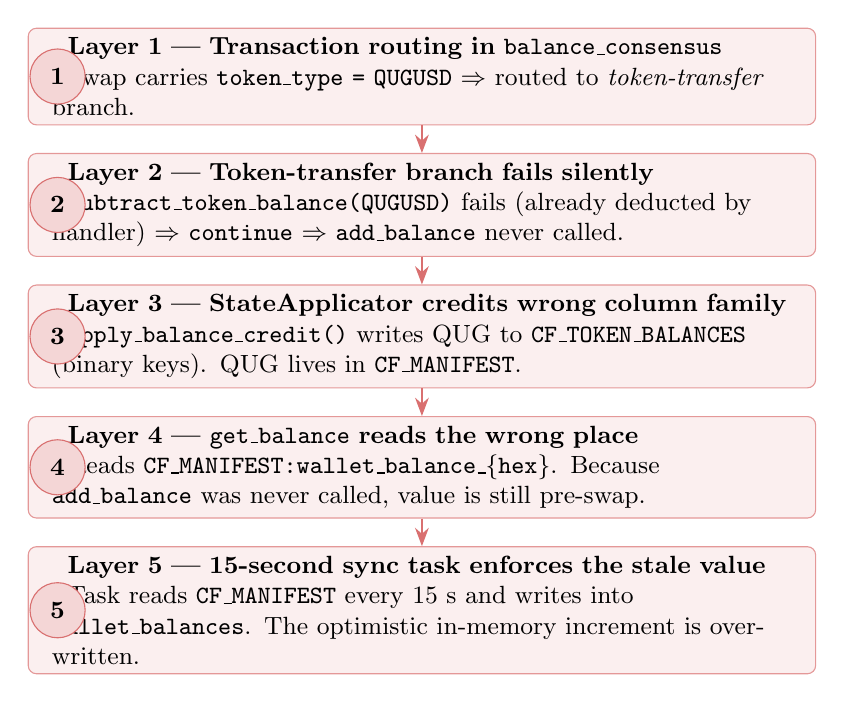
\begin{tikzpicture}[
  layer/.style={rectangle, rounded corners=3pt, draw, fill=qugred!8,
    draw=qugred!50, minimum width=10cm, minimum height=1cm,
    font=\small, align=left, text width=9.4cm, inner xsep=6pt},
  num/.style={circle, draw=qugred!70, fill=qugred!20, font=\bfseries\small,
    minimum size=0.7cm},
  arrow/.style={-{Stealth}, thick, color=qugred!70}
]
\node[layer] (L1) at (0,0) {%
  \hspace{0.2cm}\textbf{Layer 1 — Transaction routing in \texttt{balance\_consensus}}\\
  \hspace{0.2cm}\small Swap carries \texttt{token\_type = QUGUSD} $\Rightarrow$ routed to
    \emph{token-transfer} branch.};

\node[layer, below=0.35cm of L1] (L2) {%
  \hspace{0.2cm}\textbf{Layer 2 — Token-transfer branch fails silently}\\
  \hspace{0.2cm}\small \texttt{subtract\_token\_balance(QUGUSD)} fails (already deducted
    by handler) $\Rightarrow$ \texttt{continue} $\Rightarrow$ \texttt{add\_balance} never called.};

\node[layer, below=0.35cm of L2] (L3) {%
  \hspace{0.2cm}\textbf{Layer 3 — StateApplicator credits wrong column family}\\
  \hspace{0.2cm}\small \texttt{apply\_balance\_credit()} writes QUG to
    \texttt{CF\_TOKEN\_BALANCES} (binary keys).  QUG lives in \texttt{CF\_MANIFEST}.};

\node[layer, below=0.35cm of L3] (L4) {%
  \hspace{0.2cm}\textbf{Layer 4 — \texttt{get\_balance} reads the wrong place}\\
  \hspace{0.2cm}\small Reads \texttt{CF\_MANIFEST:wallet\_balance\_\{hex\}}. Because
    \texttt{add\_balance} was never called, value is still pre-swap.};

\node[layer, below=0.35cm of L4] (L5) {%
  \hspace{0.2cm}\textbf{Layer 5 — 15-second sync task enforces the stale value}\\
  \hspace{0.2cm}\small Task reads \texttt{CF\_MANIFEST} every 15 s and writes into
    \texttt{wallet\_balances}. The optimistic in-memory increment is overwritten.};

\draw[arrow] (L1.south) -- (L2.north);
\draw[arrow] (L2.south) -- (L3.north);
\draw[arrow] (L3.south) -- (L4.north);
\draw[arrow] (L4.south) -- (L5.north);

\node[num] at ($(L1.west)+(0.38,0)$) {1};
\node[num] at ($(L2.west)+(0.38,0)$) {2};
\node[num] at ($(L3.west)+(0.38,0)$) {3};
\node[num] at ($(L4.west)+(0.38,0)$) {4};
\node[num] at ($(L5.west)+(0.38,0)$) {5};
\end{tikzpicture}
\caption{The five-layer causal chain leading to the swap revert.}
\label{fig:layers}
\end{figure}

\subsection{Why the Balance Briefly Looked Correct}

The swap handler updated \texttt{wallet\_balances} (in-memory) optimistically
after calling \texttt{record\_dex\_qug\_credit}.  The frontend SSE stream picked
this up immediately.  The 15-second task then ``corrected'' the in-memory value
back to the stale on-disk value, producing the observed 2--3 minute revert.

\subsection{Timeline Visualisation}

\begin{figure}[H]
\centering
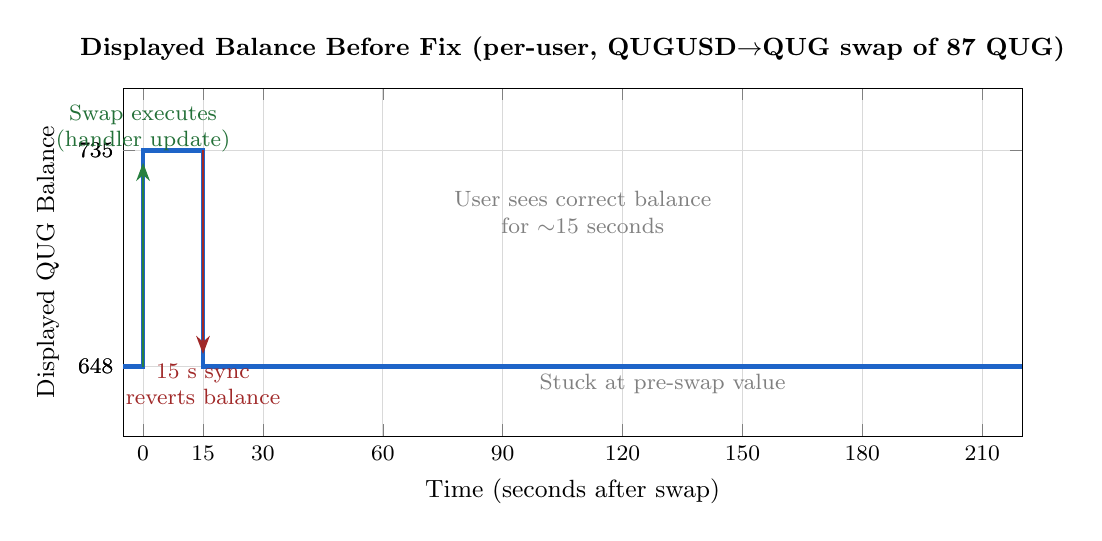
\begin{tikzpicture}
\begin{axis}[
  width=13cm, height=6cm,
  xlabel={Time (seconds after swap)},
  ylabel={Displayed QUG Balance},
  xmin=-5, xmax=220,
  ymin=620, ymax=760,
  xtick={0,15,30,60,90,120,150,180,210},
  ytick={648,735},
  yticklabels={648,735},
  extra y ticks={648,735},
  grid=both, grid style={line width=0.3pt, draw=gray!30},
  tick label style={font=\footnotesize},
  label style={font=\small},
  title style={font=\small\bfseries},
  title={Displayed Balance Before Fix (per-user, QUGUSD$\to$QUG swap of 87 QUG)},
  clip=false
]

% Pre-swap steady state
\addplot[thick, color=qugblue, const plot] coordinates {
  (-5,648)(0,648)
};

% Swap executes — immediate jump
\addplot[thick, color=quggreen, const plot] coordinates {
  (0,735)(15,735)
};

% 15-second sync reverts
\addplot[thick, color=qugred, const plot] coordinates {
  (15,648)(220,648)
};

% Combined
\addplot[ultra thick, color=qugblue, const plot, forget plot] coordinates {
  (-5,648)(0,648)(0,735)(15,735)(15,648)(220,648)
};

% Annotations
\draw[-{Stealth}, color=quggreen!80!black, thick]
  (axis cs:0,648) -- (axis cs:0,730)
  node[above, font=\footnotesize, color=quggreen!70!black, align=center]
    {Swap executes \\ (handler update)};

\draw[-{Stealth}, color=qugred!80!black, thick]
  (axis cs:15,735) -- (axis cs:15,653)
  node[below, font=\footnotesize, color=qugred!80!black, align=center]
    {15 s sync \\ reverts balance};

\node[font=\footnotesize, color=gray, align=center] at (axis cs:110,710)
  {User sees correct balance \\ for $\sim$15 seconds};
\node[font=\footnotesize, color=gray] at (axis cs:130,641)
  {Stuck at pre-swap value};

\end{axis}
\end{tikzpicture}
\caption{Balance timeline for a 87-QUG QUGUSD$\to$QUG swap before v10.5.1. The
  in-memory optimistic update is overwritten by the 15-second sync task.}
\label{fig:timeline1}
\end{figure}

% ═════════════════════════════════════════════════════════════════════════════
\section{Fix 1 — v10.5.1: Direct CF\_MANIFEST Write in Handler}
% ═════════════════════════════════════════════════════════════════════════════

The fix writes the QUG credit directly to \texttt{CF\_MANIFEST} in the HTTP
handler (synchronous with the API call), then re-reads the updated value and
stores it in the in-memory map so the 15-second sync task confirms rather than
reverts.

\begin{lstlisting}[caption={v10.5.1 handler fix — \texttt{crates/q-api-server/src/handlers.rs}},
                   label={lst:v10501}]
if to_is_qug {
    drop(token_balances);
    let wallet_hex = hex::encode(wallet_addr);
    // Step 1: Record credit counter (idempotency for restart reconciliation)
    if let Err(e) = state.storage_engine
        .record_dex_qug_credit(&wallet_hex, final_amount_out as u128).await {
        warn!("[SWAP v10.5.1] Failed to record DEX credit counter: {}", e);
    }
    // Step 2: Write QUG directly to CF_MANIFEST (same key get_balance reads)
    match state.storage_engine.add_balance(&wallet_hex, final_amount_out as u128).await {
        Ok(_) => {
            // Step 3: Re-read and sync in-memory so 15 s task confirms, not reverts
            let new_qug = state.storage_engine.get_balance(&wallet_hex).await.unwrap_or(0);
            let mut wb = state.wallet_balances.write().await;
            wb.insert(wallet_addr, new_qug);
        }
        Err(e) => { warn!("[SWAP v10.5.1] Failed to persist QUG credit: {}", e); }
    }
}
\end{lstlisting}

After this fix, the on-disk and in-memory values are consistent.  The
15-second task reads 735 QUG from disk and writes 735 QUG to memory —
confirming rather than reverting.

% ═════════════════════════════════════════════════════════════════════════════
\section{Bug 2: Post-Checkpoint DEX Credit Loss on Restart}
% ═════════════════════════════════════════════════════════════════════════════

\subsection{Why v10.5.1 Revealed This Bug}

Before v10.5.1, balances always reverted within 15 seconds.  Users never
accumulated a ``correct'' balance that a restart could destroy.  With v10.5.1,
balances persisted correctly — until the node restarted.

\subsection{The Checkpoint Mechanism}

All nodes embed a hardcoded \emph{checkpoint} at block~16,538,868
(1,326 wallets).  On startup, if the checkpoint marker
\texttt{\_\_balance\_checkpoint\_v1\_\_} is absent from the database, the node:
\begin{enumerate}
  \item Purges all \texttt{wallet\_balance\_\{hex\}} keys from \texttt{CF\_MANIFEST}
  \item Imports the 1,326 checkpoint wallet balances
  \item Replays post-checkpoint blocks (Coinbase + Transfer only — \emph{not} Swap)
  \item Runs \texttt{apply\_dex\_qug\_adjustments()} to re-credit DEX swaps
  \item Writes the marker so the restore does not repeat
\end{enumerate}

Swap transactions are intentionally excluded from post-checkpoint replay
because their state is managed by the DEX counter mechanism.  This is the
correct design — but it only works if \texttt{apply\_dex\_qug\_adjustments}
produces the right delta.

\subsection{Root Cause}

The delta formula used by \texttt{apply\_dex\_qug\_adjustments} is:

\[
  \Delta = \underbrace{(C - D)}_{\text{desired net}} -
           \underbrace{A}_{\text{previously applied}}
\]

where $C$ = \texttt{dex\_qug\_credited:\{wallet\}},
$D$ = \texttt{dex\_qug\_debited:\{wallet\}},
$A$ = \texttt{dex\_applied\_net:\{wallet\}}.

The problem was in \texttt{record\_dex\_qug\_credit} (called by the
v10.5.1 handler):

\begin{lstlisting}[caption={Broken write in \texttt{record\_dex\_qug\_credit} (pre-v10.5.2)},
                   label={lst:broken}]
// BUG: record_dex_qug_credit wrote dex_applied_net = C - D
// This told apply_dex_qug_adjustments "already applied", causing delta = 0
self.hot_db.put_sync(CF_MANIFEST, applied_net_key.as_bytes(),
    &net.to_le_bytes()).await?;
\end{lstlisting}

After a checkpoint restore:
\begin{itemize}
  \item \texttt{wallet\_balance\_} was reset to 648 (checkpoint value)
  \item \texttt{dex\_applied\_net:} = 87 \emph{survived} (checkpoint did not purge it)
  \item \texttt{dex\_qug\_credited:} = 87 (survived)
\end{itemize}

The adjustment formula then computed $\Delta = (87 - 0) - 87 = 0$, so nothing
was applied and the balance stayed at 648.

\subsection{Balance Timeline — The Visible Drop}

\begin{figure}[H]
\centering
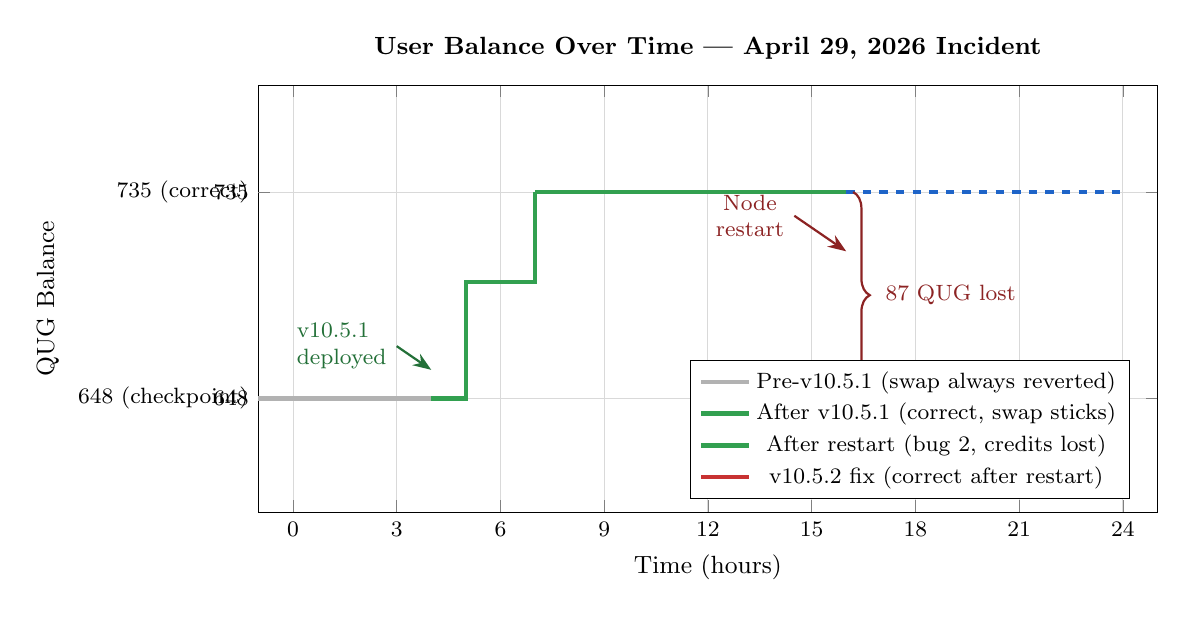
\begin{tikzpicture}
\begin{axis}[
  width=13cm, height=7cm,
  xlabel={Time (hours)},
  ylabel={QUG Balance},
  xmin=-1, xmax=25,
  ymin=600, ymax=780,
  xtick={0,3,6,9,12,15,18,21,24},
  ytick={648,735},
  yticklabels={648 (checkpoint),735 (correct)},
  extra y ticks={648,735},
  grid=both, grid style={line width=0.3pt, draw=gray!30},
  tick label style={font=\footnotesize},
  label style={font=\small},
  title style={font=\small\bfseries},
  title={User Balance Over Time --- April 29, 2026 Incident},
  clip=false,
  legend pos=south east,
  legend style={font=\footnotesize}
]

% Pre-deploy: always at 648 (swap revert bug)
\addplot[ultra thick, color=gray!60, const plot] coordinates {
  (-1,648)(4,648)
};
\addlegendentry{Pre-v10.5.1 (swap always reverted)};

% v10.5.1 deployed at t=4h: balance climbs correctly with each swap
\addplot[ultra thick, color=quggreen, const plot] coordinates {
  (4,648)(5,648)(5,697)(5,697)(7,697)(7,735)
};
\addlegendentry{After v10.5.1 (correct, swap sticks)};

% Steady at 735
\addplot[ultra thick, color=quggreen, const plot] coordinates {
  (7,735)(16,735)
};

% Restart at t=16h: balance drops to 648
\addplot[ultra thick, color=qugred, const plot] coordinates {
  (16,648)(24,648)
};
\addlegendentry{After restart (bug 2, credits lost)};

% Correct after v10.5.2
\addplot[ultra thick, color=qugblue, dashed, const plot] coordinates {
  (16,735)(24,735)
};
\addlegendentry{v10.5.2 fix (correct after restart)};

% Event annotations
\draw[{Stealth}-,thick,color=quggreen!70!black]
  (axis cs:4,660) -- (axis cs:3,670)
  node[left,font=\footnotesize,color=quggreen!70!black,align=left]{v10.5.1\\deployed};

\draw[{Stealth}-,thick,color=qugred!70!black]
  (axis cs:16,710) -- (axis cs:14.5,725)
  node[left,font=\footnotesize,align=center,color=qugred!70!black]{Node\\restart};

\draw[thick,color=qugred!70!black,decorate,
  decoration={brace,amplitude=6pt,mirror}]
  (axis cs:16.2,648) -- (axis cs:16.2,735)
  node[midway,right=8pt,font=\footnotesize,color=qugred!70!black]{87 QUG lost};

\end{axis}
\end{tikzpicture}
\caption{The observed balance trajectory on April 29, 2026. After v10.5.1 the
  swap correctly credited 87 QUG. The subsequent restart triggered a checkpoint
  restore that silently discarded those credits, returning the balance to the
  checkpoint value of 648 QUG.}
\label{fig:timeline2}
\end{figure}

% ═════════════════════════════════════════════════════════════════════════════
\section{Fix 2 — v10.5.2: Three-Part Repair}
% ═════════════════════════════════════════════════════════════════════════════

\subsection{Change 1 — Checkpoint Restore Also Resets \texttt{dex\_applied\_net}}

\begin{lstlisting}[caption={\texttt{crates/q-storage/src/lib.rs} — checkpoint restore (~line 5511)},
                   label={lst:fix1}]
// Purge on-disk balance records (as before)
let deleted = self.delete_by_prefix(b"wallet_balance_").await.unwrap_or(0);

// NEW in v10.5.2: also reset the dex_applied_net sentinel
let dex_net_purged = self.delete_by_prefix(b"dex_applied_net:").await.unwrap_or(0);
if dex_net_purged > 0 {
    warn!("[CHECKPOINT] Reset {} dex_applied_net entries - \
           adjustments will be re-applied this boot.", dex_net_purged);
}
\end{lstlisting}

After this purge, $A = 0$ for all wallets, so $\Delta = (87 - 0) - 0 = 87$
and the correct balance is restored on startup.

\subsection{Change 2 — \texttt{record\_dex\_qug\_credit} No Longer Writes \texttt{dex\_applied\_net}}

\begin{lstlisting}[caption={\texttt{crates/q-storage/src/lib.rs} — \texttt{record\_dex\_qug\_credit} (~line 9428)},
                   label={lst:fix2}]
// v10.5.2: Do NOT write dex_applied_net here.
// Only apply_dex_qug_adjustments() should set this, after checkpoint restore.
self.hot_db.put_sync(CF_MANIFEST, credit_key.as_bytes(),
    &new_credit_total.to_le_bytes()).await?;
\end{lstlisting}

This separates concerns: the handler records credits/debits;
\texttt{apply\_dex\_qug\_adjustments} is the sole authority on what has been
applied to the on-disk balance.

\subsection{Change 3 — Authoritative-Node Guard}

Epsilon is the genesis node: it has held the chain since block 0 and its
database is \emph{more authoritative than any embedded checkpoint}.  Before
v10.5.2, any restart would wipe Epsilon's live balances because the checkpoint
marker was absent.  The fix detects this situation automatically:

\begin{lstlisting}[caption={Authoritative-node guard — \texttt{lib.rs} checkpoint entry point},
                   label={lst:guard}]
// If this node already has >= checkpoint wallet count AND is past checkpoint
// height, it is the authoritative source - skip wipe, write marker.
let existing_wallets = self.hot_db
    .scan_prefix(CF_MANIFEST, b"wallet_balance_").await
    .map(|v| v.len()).unwrap_or(0);

if existing_wallets >= CHECKPOINT_WALLET_COUNT && local_height > CHECKPOINT_HEIGHT {
    warn!("[CHECKPOINT] Skipping wipe: node has {} wallets at height {} \
           (checkpoint has {} at height {}). Node is authoritative.",
          existing_wallets, local_height, CHECKPOINT_WALLET_COUNT, CHECKPOINT_HEIGHT);
    self.hot_db.put_sync(CF_MANIFEST, Self::CHECKPOINT_APPLIED_KEY,
        b"skipped-authoritative").await?;
    return Ok(());
}
\end{lstlisting}

Any node that already has at least as many wallets as the checkpoint and is
past the checkpoint height is treated as authoritative.  No environment
variable, no flag, no remembered rule.

% ═════════════════════════════════════════════════════════════════════════════
\section{Correctness Analysis}
% ═════════════════════════════════════════════════════════════════════════════

\subsection{State Table — Normal Operation (No Restart)}

\begin{center}
\begin{tabular}{lcccc}
\toprule
\textbf{Event} & \textbf{\texttt{wallet\_balance\_}} & \textbf{\texttt{dex\_credited:}} &
  \textbf{\texttt{dex\_applied\_net:}} & \textbf{In-Memory} \\
\midrule
Before swap & 648 & 0 & 0 & 648 \\
Swap (handler) & 735 (\texttt{add\_balance}) & 87 & 0 (v10.5.2) & 735 \\
15 s sync & 735 & --- & --- & 735 $\checkmark$ \\
\bottomrule
\end{tabular}
\end{center}

\subsection{State Table — After Restart with v10.5.2}

\begin{center}
\begin{tabular}{lccl}
\toprule
\textbf{Phase} & \textbf{\texttt{wallet\_balance\_}} & \textbf{\texttt{dex\_applied\_net:}} &
  \textbf{Result} \\
\midrule
Checkpoint purge & 648 (reset) & 0 (reset) & — \\
\texttt{apply\_dex\_qug\_adjustments} & $648 + 87 = 735$ & 87 & 735 $\checkmark$ \\
Second restart & 648 $\to$ $+87 = 735$ & $0 \to 87$ & 735 $\checkmark$ \\
\bottomrule
\end{tabular}
\end{center}

\subsection{Double-Credit Analysis}

Could both the handler's \texttt{add\_balance} and
\texttt{apply\_dex\_qug\_adjustments} apply the same credit?

\begin{itemize}
  \item \textbf{Same session (no restart):} \texttt{apply\_dex\_qug\_adjustments}
        runs at startup before any swaps.  The handler runs later.  The adjustment
        routine does not run again.  No double-credit.
  \item \textbf{After restart:} The checkpoint resets
        \texttt{wallet\_balance\_} to 648, wiping the handler's \texttt{add\_balance}
        write.  \texttt{apply\_dex\_qug\_adjustments} then applies $+87$.
        Net: $648 + 87 = 735$.  Correct — not a double-credit.
\end{itemize}

% ═════════════════════════════════════════════════════════════════════════════
\section{System Architecture After Fix}
% ═════════════════════════════════════════════════════════════════════════════

\begin{figure}[H]
\centering
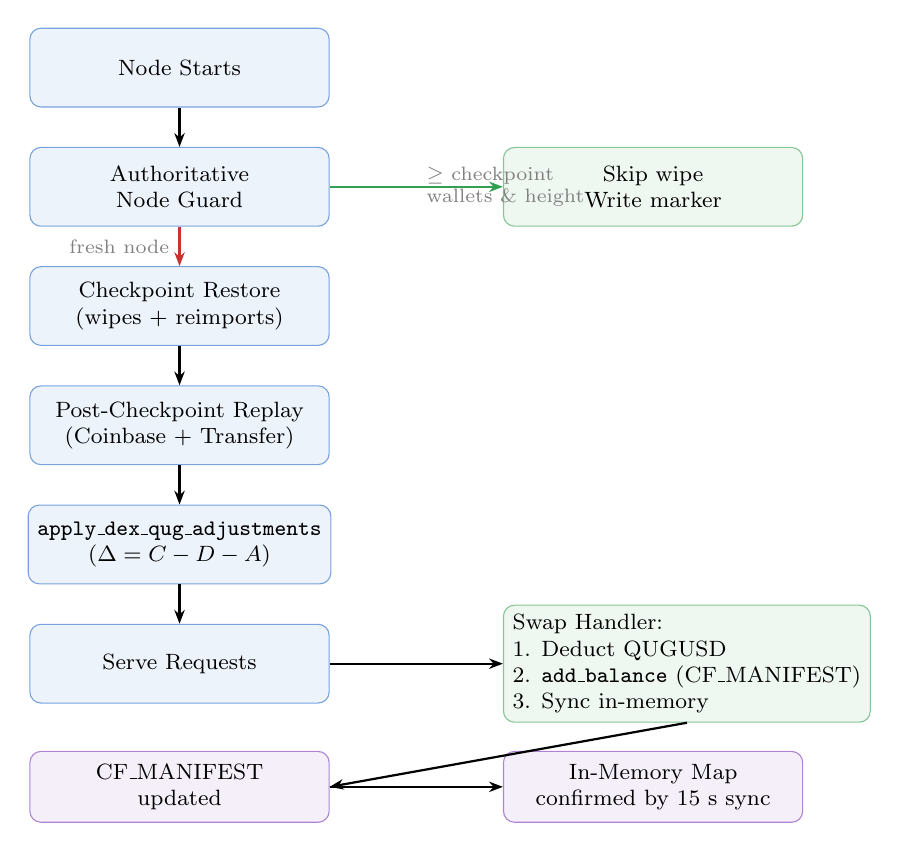
\begin{tikzpicture}[
  node distance=0.6cm and 1.8cm,
  phase/.style={rectangle, rounded corners=4pt, draw=qugblue!60,
    fill=qugblue!8, minimum width=3.8cm, minimum height=1.0cm,
    font=\footnotesize, align=center},
  store/.style={rectangle, rounded corners=4pt, draw=qugpurple!60,
    fill=qugpurple!8, minimum width=3.8cm, minimum height=0.9cm,
    font=\footnotesize, align=center},
  action/.style={-{Stealth[length=5pt]}, thick},
  label/.style={font=\scriptsize, color=gray}
]

% Startup sequence
\node[phase] (start)  {Node Starts};
\node[phase, below=0.5cm of start] (guard) {Authoritative\\Node Guard};
\node[phase, below=0.5cm of guard] (ckpt) {Checkpoint Restore\\(wipes + reimports)};
\node[phase, below=0.5cm of ckpt] (replay) {Post-Checkpoint Replay\\(Coinbase + Transfer)};
\node[phase, below=0.5cm of replay] (dex) {\texttt{apply\_dex\_qug\_adjustments}\\($\Delta = C - D - A$)};
\node[phase, below=0.5cm of dex] (serve) {Serve Requests};

% Authoritative bypass
\node[phase, right=2.2cm of guard, fill=quggreen!8, draw=quggreen!60]
  (skip) {Skip wipe\\Write marker};

% Swap path
\node[phase, right=2.2cm of serve, fill=quggreen!8, draw=quggreen!60, align=left]
  (swap) {Swap Handler:\\1. Deduct QUGUSD\\2. \texttt{add\_balance} (CF\_MANIFEST)\\3. Sync in-memory};

% Storage nodes
\node[store, below=0.6cm of serve] (cfm2) {CF\_MANIFEST\\updated};
\node[store, right=2.2cm of cfm2, align=center] (inmem2) {In-Memory Map\\confirmed by 15 s sync};

% Arrows
\draw[action] (start) -- (guard);
\draw[action, color=quggreen] (guard) -- node[right, label, align=left]{$\geq$ checkpoint\\wallets \& height} (skip);
\draw[action, color=qugred] (guard) -- node[left, label]{fresh node} (ckpt);
\draw[action] (ckpt) -- (replay);
\draw[action] (replay) -- (dex);
\draw[action] (dex) -- (serve);
\draw[action] (serve) -- (swap);
\draw[action] (swap.south) -- (cfm2.east);
\draw[action] (cfm2) -- (inmem2);

\end{tikzpicture}
\caption{Startup and swap flow after v10.5.2. Authoritative nodes bypass the
  checkpoint wipe automatically. Fresh syncing nodes apply the checkpoint, then
  the DEX adjustment routine re-credits swap history correctly.}
\label{fig:arch}
\end{figure}

% ═════════════════════════════════════════════════════════════════════════════
\section{Impact Assessment}
% ═════════════════════════════════════════════════════════════════════════════

\subsection{What Was Lost}

\begin{center}
\begin{tabular}{lcc}
\toprule
\textbf{User} & \textbf{Expected Balance} & \textbf{Balance After Restart} \\
\midrule
Primary affected user & 735 QUG & 648 QUG \\
\textbf{Difference} & \multicolumn{2}{c}{\textbf{87 QUG lost ($\approx$ 1 day of mining rewards)}} \\
\bottomrule
\end{tabular}
\end{center}

The 87 QUG difference represents native QUG received via QUGUSD$\to$QUG swaps
that were correctly persisted by v10.5.1 but not re-applied after the restart
because of the broken \texttt{dex\_applied\_net} accounting.

\subsection{Why This Was Not Auto-Recoverable Under v10.5.1}

The checkpoint at height 16,538,868 authoritatively sets the starting balances.
The post-checkpoint replay excludes swap transactions.  With the pre-v10.5.2
code, the only mechanism to restore swap credits after a restart was
\texttt{apply\_dex\_qug\_adjustments}, and that mechanism was neutralised by the
incorrect \texttt{dex\_applied\_net} write.  The credits were silently lost on
every restart while v10.5.1 was deployed.

\subsubsection*{Who Is Affected and When}

\begin{itemize}
  \item \textbf{Nodes that restarted between v10.5.1 and v10.5.2}: swap-derived
        QUG credits accumulated after the checkpoint were lost.  87 QUG was lost
        in the documented case.
  \item \textbf{Nodes that ran v10.5.1 continuously without restart}: balances
        were correct in \texttt{CF\_MANIFEST}; no loss occurred.
  \item \textbf{Any node restarting after v10.5.2}: \texttt{apply\_dex\_qug\_adjustments}
        correctly reapplies all swap credits; no intervention needed.
\end{itemize}

The loss was therefore limited to the window between the v10.5.1 deploy and the
v10.5.2 deploy on April 29, 2026, and only affected nodes restarted in that window.

\subsection{Affected Versions}

\begin{center}
\begin{tabular}{lll}
\toprule
\textbf{Version} & \textbf{Swap Revert Bug} & \textbf{Restart Credit Loss} \\
\midrule
$\leq$ v10.4.x & \textcolor{qugred}{Present} & Hidden (swap always reverted) \\
v10.5.1        & \textcolor{quggreen}{Fixed} & \textcolor{qugred}{Revealed \& present} \\
v10.5.2        & \textcolor{quggreen}{Fixed} & \textcolor{quggreen}{Fixed} \\
\bottomrule
\end{tabular}
\end{center}

% ═════════════════════════════════════════════════════════════════════════════
\section{Remaining Risks and Open Issues}
% ═════════════════════════════════════════════════════════════════════════════

\begin{noticebox}[R1 — DEX Debits After Checkpoint Also Not Replayed]
QUG$\to$QUGUSD debits (the debit side) are also excluded from post-checkpoint
replay.  However, \texttt{atomic\_subtract\_and\_record\_dex\_debit} already
writes directly to \texttt{CF\_MANIFEST} — mirroring v10.5.1 for credits.
Debits survive correctly in \texttt{CF\_MANIFEST}.  After a checkpoint restore,
\texttt{apply\_dex\_qug\_adjustments} subtracts the debit delta — which is
correct.

\textbf{Action:} Verify \texttt{atomic\_subtract\_and\_record\_dex\_debit} does
\emph{not} write \texttt{dex\_applied\_net} (if it does, the same bug exists on
the debit side).
\end{noticebox}

\medskip

\begin{infobox}[R2 — Checkpoint Staleness]
The checkpoint is hardcoded at block 16,538,868.  As the chain grows, the
post-checkpoint replay window grows with it.  Each restart currently replays
$\sim$151,000 blocks of Coinbase + Transfer transactions.  This replay time
will grow indefinitely until a new checkpoint is embedded.

\textbf{Recommendation:} Update \texttt{CHECKPOINT\_DATA} to a more recent height
in the next planned maintenance release.
\end{infobox}

\medskip

\begin{infobox}[R3 — Swap Transactions Excluded from Replay]
The fundamental design gap is that swap transactions are excluded from
post-checkpoint replay.  Any QUG state from swaps exists \emph{only} in the
DEX counter mechanism.  If the counter data is ever lost or corrupted, the
credits are unrecoverable from chain history.

\textbf{Long-term recommendation:} Include swap transactions in the
post-checkpoint replay, or update the checkpoint more frequently.
\end{infobox}

\medskip

\begin{noticebox}[R4 — No Atomicity Between QUGUSD Deduction and QUG Credit]
The swap handler calls \texttt{subtract\_token\_balance} (QUGUSD deduction) and
then \texttt{add\_balance} (QUG credit) as two separate async operations with no
two-phase commit.  If the process crashes between them, the user loses QUGUSD
without receiving QUG.  The DEX counter
(\texttt{record\_dex\_qug\_credit}) provides \emph{partial} idempotency on
restart, but only if the credit counter write also succeeded before the crash.

\textbf{Recommendation:} Write QUGUSD deduction, QUG credit, and counter update
as a single RocksDB \texttt{WriteBatch} to make the operation atomic with
respect to crashes.
\end{noticebox}

\medskip

\begin{noticebox}[R5 — Checkpoint Marker Is a Single Deletable Key]
The guard against double-restore is a single key
\texttt{\_\_balance\_checkpoint\_v1\_\_} in \texttt{CF\_MANIFEST}.  If deleted
accidentally (manual DB operation, prefix scan gone wrong), the next restart will
trigger a full balance wipe.  There is no secondary marker, read-only mode, or
pre-restore sanity check.

\textbf{Recommendation:} Write the marker to two independent locations (e.g.\
both \texttt{CF\_MANIFEST} and \texttt{CF\_META}); require both to be present
before skipping the restore.
\end{noticebox}

\medskip

\begin{infobox}[R6 — Authoritative-Node Guard Uses Wallet Count, Not Height Alone]
The guard condition is \texttt{existing\_wallets >= CHECKPOINT\_WALLET\_COUNT \&\& local\_height > CHECKPOINT\_HEIGHT}.  A node that has been synced only up to the
checkpoint height might satisfy the wallet count check while having incorrect or
incomplete post-checkpoint state.  The condition is sufficient for the known
genesis node scenario but not for all possible node states.

\textbf{Safer condition:} \texttt{local\_height > CHECKPOINT\_HEIGHT} alone
(i.e.\ any node that has advanced past the checkpoint is treated as having
applied it); or additionally check that the sum of all \texttt{wallet\_balance\_}
values differs from the checkpoint total (indicating live transactions occurred).
\end{infobox}

% ═════════════════════════════════════════════════════════════════════════════
\section{Summary of Changes}
% ═════════════════════════════════════════════════════════════════════════════

\begin{center}
\begin{tabularx}{\textwidth}{lXl}
\toprule
\textbf{File} & \textbf{Change} & \textbf{Risk} \\
\midrule
\texttt{handlers.rs} &
  \texttt{add\_balance} + in-memory sync after QUGUSD$\to$QUG swap &
  Medium \\
\texttt{lib.rs:5511} &
  Checkpoint restore purges \texttt{dex\_applied\_net:} keys &
  Low \\
\texttt{lib.rs:9428} &
  \texttt{record\_dex\_qug\_credit} no longer writes \texttt{dex\_applied\_net} &
  Low \\
\texttt{lib.rs:5489} &
  Authoritative-node guard skips checkpoint wipe automatically &
  Low \\
\texttt{Cargo.toml} &
  Version bump 10.5.0 $\to$ 10.5.1 $\to$ 10.5.2 &
  None \\
\bottomrule
\end{tabularx}
\end{center}

\bigskip

\begin{fixbox}[Deploy Note]
Nodes that restarted between v10.5.1 and v10.5.2 lost swap-derived credits;
those credits are \textbf{not} automatically restored without a further restart
under v10.5.2 (the DEX counter data survives and is correct — a restart is all
that is needed).  Nodes that did not restart while v10.5.1 was deployed retain
the correct balance and require no action.  The authoritative-node guard ensures
the genesis node (Epsilon) is protected from checkpoint wipes on all future
restarts.
\end{fixbox}

% ═════════════════════════════════════════════════════════════════════════════
\section{Conclusion}
% ═════════════════════════════════════════════════════════════════════════════

Two compounding bugs caused users to observe their QUG balances decrease
without performing any transactions.  The root cause in both cases was a
disconnect between where QUG credits were recorded and where the authoritative
balance lived in the storage engine.

The v10.5.1 fix correctly routes QUGUSD$\to$QUG swap credits to
\texttt{CF\_MANIFEST} at transaction time.  The v10.5.2 fix ensures that the
startup reconciliation routine always has accurate data to work from after a
checkpoint restore, and that the genesis node is never subjected to a
checkpoint wipe it does not need.

We are committed to transparency.  If you observed a balance change that you
cannot account for, please contact the development team.  The period of
incorrectness was the time between the v10.5.1 deploy and the subsequent
restart on April 29, 2026.

% ═════════════════════════════════════════════════════════════════════════════
\appendix
\section{Lessons Learned \& Test Plan}
% ═════════════════════════════════════════════════════════════════════════════

\subsection{Lessons Learned}

\begin{enumerate}

\item \textbf{Eventual-consistency paths need end-to-end timer tests.}\\
  The 15-second sync task was known; the swap handler touched the same
  in-memory map.  A test of the form ``swap → sleep 16 s → assert balance''
  would have caught Bug 1 immediately.  Any feature that writes to memory and
  relies on a background task to persist must have a test that waits for that
  task.

\item \textbf{Every fix needs a restart regression test.}\\
  v10.5.1 wrote to \texttt{CF\_MANIFEST}.  The natural follow-on test is:
  ``write → restart with checkpoint → assert balance''.  Bug 2 would have been
  found before deployment.

\item \textbf{Checkpoint purge lists are an explicit contract.}\\
  The checkpoint restore deleted \texttt{wallet\_balance\_*} but left
  \texttt{dex\_applied\_net:*} intact.  The purge list must be treated as an
  explicit whitelist: any key namespace that influences balance state must appear
  in it.  Treat a missing entry as a bug, not an oversight.

\item \textbf{Two separate async writes are not atomic.}\\
  Deducting QUGUSD and crediting QUG are two RocksDB writes.  A crash between
  them leaves the chain in an inconsistent state.  Financial operations must be
  composed into a single \texttt{WriteBatch}.

\item \textbf{Authoritative-node detection should not depend on wallet count.}\\
  Comparing wallet count to a hardcoded checkpoint constant is fragile.  A
  single key recording ``highest height reached'' would give a cleaner,
  monotonic guard.

\item \textbf{The DEX counter mechanism is not a substitute for block replay.}\\
  Swap state that lives only in metadata keys is unrecoverable from chain
  history.  Long-term, swap transactions must be included in post-checkpoint
  replay, or the checkpoint must be updated frequently enough that the
  counter-only window is negligible.

\end{enumerate}

\subsection{Test Plan — What Would Have Prevented These Bugs}

\begin{center}
\begin{tabularx}{\textwidth}{p{3.2cm}Xp{2.2cm}}
\toprule
\textbf{Test ID} & \textbf{Description} & \textbf{Bug Caught} \\
\midrule
T-01 & Perform QUGUSD$\to$QUG swap. Wait 20 s. Assert displayed QUG balance equals pre-swap plus swap amount. &
  Bug 1 \\
T-02 & Perform swap (T-01). Read \texttt{CF\_MANIFEST:wallet\_balance\_\{hex\}} directly. Assert equals expected. &
  Bug 1, Layer 4 \\
T-03 & Perform swap. Restart node. Assert balance is restored from disk, not reverted to pre-swap value. &
  Bug 2 \\
T-04 & Perform swap. Restart node with embedded checkpoint (simulate fresh sync). Assert \texttt{apply\_dex\_qug\_adjustments} adds correct delta. &
  Bug 2 (root) \\
T-05 & Perform swap. Read \texttt{dex\_applied\_net:\{wallet\}}. Assert it is \textbf{zero} (not set by handler). Restart. Assert non-zero delta applied. &
  Bug 2 (wrong write) \\
T-06 & Insert test wallet data exceeding checkpoint. Restart. Assert checkpoint restore is \textbf{skipped}. Assert balances unchanged. &
  Epsilon wipe \\
T-07 & Delete \texttt{\_\_balance\_checkpoint\_v1\_\_} key manually. Restart. Assert node does \textbf{not} wipe a populated authoritative DB. &
  R5 (marker loss) \\
T-08 & Simulate crash between \texttt{subtract\_token\_balance} and \texttt{add\_balance} (kill process mid-handler). Restart. Assert QUGUSD deduction is rolled back or QUG credit is applied, not both half-done. &
  R4 (atomicity) \\
T-09 & Run 100 QUGUSD$\to$QUG swaps. Compute expected total from swap amounts. Assert \texttt{dex\_qug\_credited:\{wallet\}} equals sum. Restart with checkpoint. Assert balance = checkpoint + total delta. &
  Multi-swap accumulation (R2) \\
T-10 & Assert \texttt{atomic\_subtract\_and\_record\_dex\_debit} does \textbf{not} write \texttt{dex\_applied\_net}. &
  R1 (debit side) \\
\bottomrule
\end{tabularx}
\end{center}

\bigskip

\begin{infobox}[Priority Order for Implementation]
Run T-01 through T-05 immediately (they directly test the v10.5.1/v10.5.2 fixes
and regressions).  T-06 and T-07 protect the authoritative-node guard.  T-08
and T-09 cover the remaining architectural risks.  T-10 should be a static
assertion checked by CI.
\end{infobox}

\bigskip

\begin{center}
{\small\textcolor{gray}{%
Q-NarwhalKnight Development Team $\cdot$ April 29, 2026 $\cdot$
\href{https://quillon.xyz}{quillon.xyz}%
}}
\end{center}

\end{document}
